%% Time-stamp: <2019-02-01 09:10:32 (marc)>
\documentclass[xcolor=x11names,compress,mathserif]{beamer}

\newcommand\hmmax{0}
\newcommand\bmmax{0}

\usepackage{../includes/MarkMathCmds}

\newcommand{\hackspace}{\hspace{4.2mm}}
\newcommand{\showstudent}[1]{}





% talk/author information
\newcommand{\authorname}{Mark van der Wilk}
\newcommand{\authoremail}{m.vdwilk@imperial.ac.uk}
\newcommand{\authoraffiliation}{
 Department of Computing\\Imperial
  College London}
\newcommand{\authortwitter}{markvanderwilk}
\newcommand{\slidesettitle}{\imperialBlue{Markov Chain Monte Carlo}}
\newcommand{\footertitle}{Markov Chain Monte Carlo}
\newcommand{\location}{Imperial College London}
\newcommand{\talkDate}{{February 24, 2023}}


\date{\imperialGray{\talkDate}}




% load defaults
\selectcolormodel{rgb}
\usepackage{ifxetex,ifluatex}
\newif\ifxetexorluatex
\ifxetex
  \xetexorluatextrue
\else
  \ifluatex
    \xetexorluatextrue
  \else
    \xetexorluatexfalse
  \fi
\fi

\usepackage{textpos}
%\usepackage{arabtex}
\usepackage{tikz}
\usetikzlibrary{decorations.markings}
\usetikzlibrary{arrows}
\usetikzlibrary{shapes}
\usetikzlibrary{plotmarks}
\usetikzlibrary{mindmap,trees,backgrounds}

\tikzstyle{every picture}+=[remember picture]

%\usepackage{movie15}
% \usepackage{pdfpages}
%\usepackage{xmpmulti}

\usepackage{anyfontsize}
\usepackage{wrapfig}
\usepackage{animate}
\usepackage{multirow}
\usepackage{multimedia}
\usepackage{xmpmulti}
%\usepackage[latin9]{inputenc}
\usepackage[english]{babel}
\usepackage{scalefnt}
\usepackage{verbatim}
\usepackage{url}
% \usepackage{pgf,pgfarrows,pgfnodes}
\usepackage{textpos}
\usepackage[tight,ugly]{units}
\usepackage{url}
\usepackage{bbm}
\usepackage[english]{babel}
\usepackage{fancyhdr}
\usepackage{bm} % correct bold symbols, like \bm
\usepackage{amsmath}
\usepackage{amsfonts}
\usepackage{amssymb}
\usepackage{mathrsfs}
\usepackage{mathtools}
\usepackage{color}
\usepackage{cancel}
\usepackage{algorithm}
\usepackage{algpseudocode}
\usepackage{mathrsfs}
\usepackage{listings}
\usepackage{graphicx} % for pdf, bitmapped graphics files
\usepackage{mathtools}
\usepackage{units}
\usepackage{subfig}
\usepackage{enumerate}
\usepackage{natbib}
\usepackage{dsfont}


\ifxetexorluatex
\usepackage{fontspec}
\setmainfont[Scale=0.8]{OpenDyslexic-Regular}
\else
\usefonttheme{professionalfonts}
\fi

\renewcommand{\vec}[1]{{\boldsymbol{{#1}}}} % vector
\newcommand{\mat}[1]{{\boldsymbol{{#1}}}} % matrix
% \newcommand{\KL}[2]{\mathrm{KL}(#1\|#2)} % KL divergence
\newcommand{\R}[0]{\mathds{R}} % real numbers
\newcommand{\Z}[0]{\mathds{Z}} % integers
\newcommand{\tr}[0]{\text{tr}} % trace
% \newcommand{\inv}{^{-1}}
% \DeclareMathOperator*{\diag}{diag}
\newcommand{\E}{\mathds{E}} % expectation
\newcommand{\var}{\mathds{V}}
\newcommand{\gauss}[2]{\mathcal{N}\big(#1,\,#2\big)}
\newcommand{\gaussx}[3]{\mathcal{N}\big(#1\,|\,#2,\,#3\big)}
\newcommand{\gaussBig}[2]{\mathcal{N}\left(#1,\,#2\right)}
\newcommand{\gaussxBig}[3]{\mathcal{N}\left(#1\,\left|\,#2,\,#3\right.\right)}
\newcommand{\Ber}[0]{\mathrm{Ber}} % Bernoulli distribution
\DeclareMathOperator{\cov}{Cov}
\ifxetexorluatex
\renewcommand{\T}[0]{^\top}
\renewcommand{\d}[0]{\text{d}} % derivative
\else
\newcommand{\T}[0]{^\top}
\renewcommand{\d}[0]{\text{d}} % derivative
\fi
% calculus
\newcommand{\pdiff}[1]{\frac{\partial}{\partial #1}}
\newcommand{\pdiffF}[2]{\frac{\partial #1}{\partial #2}}
\newcommand{\diffF}[2]{\frac{{\d}#1}{{\d}#2}}
\newcommand{\diffFII}[2]{\frac{{\d}^2 #1}{{\d}#2^2}}
\newcommand{\diff}[1]{\frac{{\d}}{{\d}#1}}
\newcommand{\diffII}[1]{\frac{{\d}^2}{{\d}#1^2}}
\newcommand{\class}[0]{\mathcal{C}}

\newcommand{\idx}[1]{^{(#1)}}
% \newcommand{\norm}[1]{\left\|#1\right\|}
\newcommand{\proj}[1]{\tilde{#1}}
\newcommand{\pcacoord}{z}
\newcommand{\pcacoordnew}{\zeta}
\newcommand{\latent}{z}
% \newcommand{\given}{\,|\,}
\newcommand{\genset}[1]{\mathrm{span}[#1]} % generating set
\newcommand{\set}[1]{\mathcal{#1}} % set
\newcommand{\fixgmfont}[1]{\scalebox{0.8}{#1}}



\usepackage{pifont}% http://ctan.org/pkg/pifont
\newcommand{\cmark}{{\color{green!40!black}\ding{51}}}%
\newcommand{\xmark}{{\color{red}\ding{55}}}%
\newcommand{\green}[1]{{\bf{\textcolor{green}{#1}}}}
\newcommand{\red}[1]{{\bf{\textcolor{red}{#1}}}}

\newcommand<>\red[1]{{\color#2[rgb]{1,0,0}#1}}
\newcommand<>\blue[1]{{\color#2[rgb]{0,0,1}#1}}
\newcommand<>\yellow[1]{{\color#2{camyellow}#1}}
\newcommand<>\green[1]{{\color#2[rgb]{0,0.6,0.0}#1}}
\newcommand<>\violet[1]{{\color#2[rgb]{0.6,0,0.6}#1}}
\newcommand<>\orange[1]{{\color#2[rgb]{1,0.5,0}#1}}
\newcommand<>\black[1]{{\color#2[rgb]{0,0,0}#1}}
\newcommand<>\steel[1]{{\color#2[rgb]{0,0,0.8}#1}}
\newcommand<>\darkblue[1]{{\color#2[rgb]{0,0,0.6}#1}}
\newcommand<>\lightblue[1]{{\color#2[rgb]{0.4,0.4,0.7}#1}}
\newcommand<>\gray[1]{{\color#2[rgb]{0.4,0.4,0.4}#1}}
\newcommand<>\greenish[1]{{\color#2[rgb]{0.45, 0.66, 0.45}#1}}
\newcommand<>\redish[1]{{\color#2[rgb]{0.7843    0.3706    0.3706}#1}}
\definecolor{redishTIKZ}{rgb}{0.7843, 0.3706, 0.3706}
\definecolor{imperialBlue}{rgb}{0.058, 0.219, 0.418}
\definecolor{aimsbrown}{rgb}{0.539, 0.117, 0.015}
% \definecolor{imperialGray}{rgb}{0.414, 0.488, 0.671 }
\definecolor{imperialGray}{RGB}{109,153, 204}
\definecolor{aimslightbrown}{RGB}{138,88,84}
\newcommand<>\imperialBlue[1]{{\color#2[rgb]{0.058, 0.219, 0.418}#1}}
\newcommand<>\aimsbrown[1]{{\color#2[rgb]{0.539, 0.117, 0.015}#1}}
%\newcommand<>\imperialGray[1]{{\color#2[rgb]{0.414, 0.488, 0.671}#1}}
\newcommand<>\imperialGray[1]{{\color#2[RGB]{109,153, 204}#1}}
\newcommand<>\aimslightbrown[1]{{\color#2[RGB]{138,88,84}#1}}
\newcommand<>\lightgray[1]{{\color#2[rgb]{0.8,0.8,0.8}#1}}
%\newcommand<>\highlightcolor[1]{{\color#2[rgb]{0,0,1}#1}}
\newcommand{\highlight}[1]{{\bf\steel{#1}}}
%\newcommand{\newblock}[0]{}

%\newcommand{\arrow}[0]{\includegraphics[height=5pt]{./figures/arrow}\hspace{3pt}}

\renewcommand{\emph}[1]{\textbf{\steel{{#1}}}}

\renewcommand{\alert}[1]{{\bf\red{{#1}}}}

\newcommand{\arrow}{
\begin{tikzpicture}
\draw [black!40!green, fill=black!40!green] (0,-0.12) -- (0,0.12) --
(0.15,0);
\draw [black!40!green, fill=black!40!green] (0.15,-0.12) -- (0.15,0.12) --
(0.3,0); 
\end{tikzpicture}
}

\geometry{left=0.45cm,top=0cm,right=0.45cm}


\newcommand{\logoimagepath}{./figures/imperial}
\newcommand{\highlightcolor}{blue!80!black}
%\newcommand{\headbarcolor}{imperialBlue}
\newcommand{\headbarcolor}{imperialBlue}
\institute{}

\newcommand{\coursetitle}{}

\newcommand{\slidesetsubtitle}{}
\newcommand{\slidesetnumber}{01}
\usefonttheme{professionalfonts}


\usetikzlibrary{decorations.fractals}
% tikzlibrary.code.tex
%
% Copyright 2010-2011 by Laura Dietz
% Copyright 2012 by Jaakko Luttinen
%
% The MIT License
%
% See LICENSE file for more details.

% Load other libraries
\usetikzlibrary{shapes}
\usetikzlibrary{fit}
\usetikzlibrary{chains}
\usetikzlibrary{arrows}

% Latent node
\tikzstyle{latent} = [circle,fill=white,draw=black,inner sep=1pt,
minimum size=20pt, font=\fontsize{10}{10}\selectfont, node distance=1]
% Observed node
\tikzstyle{obs} = [latent,fill=gray!25]
% Constant node
\tikzstyle{const} = [rectangle, inner sep=0pt, node distance=1]
% Factor node
\tikzstyle{factor} = [rectangle, fill=black,minimum size=5pt, inner
sep=0pt, node distance=0.4]
% Deterministic node
\tikzstyle{det} = [latent, diamond]

% Plate node
\tikzstyle{plate} = [draw, rectangle, rounded corners, fit=#1]
% Invisible wrapper node
\tikzstyle{wrap} = [inner sep=0pt, fit=#1]
% Gate
\tikzstyle{gate} = [draw, rectangle, dashed, fit=#1]

% Caption node
\tikzstyle{caption} = [font=\footnotesize, node distance=0] %
\tikzstyle{plate caption} = [caption, node distance=0, inner sep=0pt,
below left=5pt and 0pt of #1.south east] %
\tikzstyle{factor caption} = [caption] %
\tikzstyle{every label} += [caption] %

%\pgfdeclarelayer{b}
%\pgfdeclarelayer{f}
%\pgfsetlayers{b,main,f}

% \factoredge [options] {inputs} {factors} {outputs}
\newcommand{\factoredge}[4][]{ %
  % Connect all nodes #2 to all nodes #4 via all factors #3.
  \foreach \f in {#3} { %
    \foreach \x in {#2} { %
      \path (\x) edge[-,#1] (\f) ; %
      %\draw[-,#1] (\x) edge[-] (\f) ; %
    } ;
    \foreach \y in {#4} { %
      \path (\f) edge[->, >={triangle 45}, #1] (\y) ; %
      %\draw[->,#1] (\f) -- (\y) ; %
    } ;
  } ;
}

% \edge [options] {inputs} {outputs}
\newcommand{\edge}[3][]{ %
  % Connect all nodes #2 to all nodes #3.
  \foreach \x in {#2} { %
    \foreach \y in {#3} { %
      \path (\x) edge [->, >={triangle 45}, #1] (\y) ;%
      %\draw[->,#1] (\x) -- (\y) ;%
    } ;
  } ;
}

% \factor [options] {name} {caption} {inputs} {outputs}
\newcommand{\factor}[5][]{ %
  % Draw the factor node. Use alias to allow empty names.
  \node[factor, label={[name=#2-caption]#3}, name=#2, #1,
  alias=#2-alias] {} ; %
  % Connect all inputs to outputs via this factor
  \factoredge {#4} {#2-alias} {#5} ; %
}

% \plate [options] {name} {fitlist} {caption}
\newcommand{\plate}[4][]{ %
  \node[wrap=#3] (#2-wrap) {}; %
  \node[plate caption=#2-wrap] (#2-caption) {#4}; %
  \node[plate=(#2-wrap)(#2-caption), #1] (#2) {}; %
}

% \gate [options] {name} {fitlist} {inputs}
\newcommand{\gate}[4][]{ %
  \node[gate=#3, name=#2, #1, alias=#2-alias] {}; %
  \foreach \x in {#4} { %
    \draw [-*,thick] (\x) -- (#2-alias); %
  } ;%
}

% \vgate {name} {fitlist-left} {caption-left} {fitlist-right}
% {caption-right} {inputs}
\newcommand{\vgate}[6]{ %
  % Wrap the left and right parts
  \node[wrap=#2] (#1-left) {}; %
  \node[wrap=#4] (#1-right) {}; %
  % Draw the gate
  \node[gate=(#1-left)(#1-right)] (#1) {}; %
  % Add captions
  \node[caption, below left=of #1.north ] (#1-left-caption)
  {#3}; %
  \node[caption, below right=of #1.north ] (#1-right-caption)
  {#5}; %
  % Draw middle separation
  \draw [-, dashed] (#1.north) -- (#1.south); %
  % Draw inputs
  \foreach \x in {#6} { %
    \draw [-*,thick] (\x) -- (#1); %
  } ;%
}

% \hgate {name} {fitlist-top} {caption-top} {fitlist-bottom}
% {caption-bottom} {inputs}
\newcommand{\hgate}[6]{ %
  % Wrap the left and right parts
  \node[wrap=#2] (#1-top) {}; %
  \node[wrap=#4] (#1-bottom) {}; %
  % Draw the gate
  \node[gate=(#1-top)(#1-bottom)] (#1) {}; %
  % Add captions
  \node[caption, above right=of #1.west ] (#1-top-caption)
  {#3}; %
  \node[caption, below right=of #1.west ] (#1-bottom-caption)
  {#5}; %
  % Draw middle separation
  \draw [-, dashed] (#1.west) -- (#1.east); %
  % Draw inputs
  \foreach \x in {#6} { %
    \draw [-*,thick] (\x) -- (#1); %
  } ;%
}


% Copyright (C) 2016  Joseph Rabinoff

% ipe2tikz is free software; you can redistribute it and/or modify it under
% the terms of the GNU General Public License as published by the Free
% Software Foundation; either version 3 of the License, or (at your option)
% any later version.

% ipe2tikz is distributed in the hope that it will be useful, but WITHOUT ANY
% WARRANTY; without even the implied warranty of MERCHANTABILITY or FITNESS
% FOR A PARTICULAR PURPOSE.  See the GNU General Public License for more
% details.

% You should have received a copy of the GNU General Public License along with
% ipe2tikz; if not, you can find it at "http://www.gnu.org/copyleft/gpl.html",
% or write to the Free Software Foundation, Inc., 675 Mass Ave, Cambridge, MA
% 02139, USA.


% ipe compatibility TikZ styles

\usetikzlibrary{arrows.meta}

\makeatletter

% These should behave almost exactly like ipe arrows.  They disable correcting
% for the miter length and line width.  This is important for visual consistency
% with ipe, since ipe arrows get much larger when the line width is increased.
% They also use the line join and cap styles from the main path.  These are very
% simple arrows: there is no harpoon version, and the convex hull computation is
% sloppy.

\pgfdeclarearrow{
  name = ipe _linear,
  defaults = {
    length = +1bp,
    width  = +.666bp,
    line width = +0pt 1,
  },
  setup code = {
    % Control points
    \pgfarrowssetbackend{0pt}
    \pgfarrowssetvisualbackend{
      \pgfarrowlength\advance\pgf@x by-.5\pgfarrowlinewidth}
    \pgfarrowssetlineend{\pgfarrowlength}
    \ifpgfarrowreversed
      \pgfarrowssetlineend{\pgfarrowlength\advance\pgf@x by-.5\pgfarrowlinewidth}
    \fi
    \pgfarrowssettipend{\pgfarrowlength}
    % Convex hull
    \pgfarrowshullpoint{\pgfarrowlength}{0pt}
    \pgfarrowsupperhullpoint{0pt}{.5\pgfarrowwidth}
    % The following are needed in the code:
    \pgfarrowssavethe\pgfarrowlinewidth
    \pgfarrowssavethe\pgfarrowlength
    \pgfarrowssavethe\pgfarrowwidth
  },
  drawing code = {
    \pgfsetdash{}{+0pt}
    \ifdim\pgfarrowlinewidth=\pgflinewidth\else\pgfsetlinewidth{+\pgfarrowlinewidth}\fi
    \pgfpathmoveto{\pgfqpoint{0pt}{.5\pgfarrowwidth}}
    \pgfpathlineto{\pgfqpoint{\pgfarrowlength}{0pt}}
    \pgfpathlineto{\pgfqpoint{0pt}{-.5\pgfarrowwidth}}
    \pgfusepathqstroke
  },
  parameters = {
    \the\pgfarrowlinewidth,%
    \the\pgfarrowlength,%
    \the\pgfarrowwidth,%
  },
}


\pgfdeclarearrow{
  name = ipe _pointed,
  defaults = {
    length = +1bp,
    width  = +.666bp,
    inset  = +.2bp,
    line width = +0pt 1,
  },
  setup code = {
    % Control points
    \pgfarrowssetbackend{0pt}
    \pgfarrowssetvisualbackend{\pgfarrowinset}
    \pgfarrowssetlineend{\pgfarrowinset}
    \ifpgfarrowreversed
      \pgfarrowssetlineend{\pgfarrowlength}
    \fi
    \pgfarrowssettipend{\pgfarrowlength}
    % Convex hull
    \pgfarrowshullpoint{\pgfarrowlength}{0pt}
    \pgfarrowsupperhullpoint{0pt}{.5\pgfarrowwidth}
    \pgfarrowshullpoint{\pgfarrowinset}{0pt}
    % The following are needed in the code:
    \pgfarrowssavethe\pgfarrowinset
    \pgfarrowssavethe\pgfarrowlinewidth
    \pgfarrowssavethe\pgfarrowlength
    \pgfarrowssavethe\pgfarrowwidth
  },
  drawing code = {
    \pgfsetdash{}{+0pt}
    \ifdim\pgfarrowlinewidth=\pgflinewidth\else\pgfsetlinewidth{+\pgfarrowlinewidth}\fi
    \pgfpathmoveto{\pgfqpoint{\pgfarrowlength}{0pt}}
    \pgfpathlineto{\pgfqpoint{0pt}{.5\pgfarrowwidth}}
    \pgfpathlineto{\pgfqpoint{\pgfarrowinset}{0pt}}
    \pgfpathlineto{\pgfqpoint{0pt}{-.5\pgfarrowwidth}}
    \pgfpathclose
    \ifpgfarrowopen
      \pgfusepathqstroke
    \else
      \ifdim\pgfarrowlinewidth>0pt\pgfusepathqfillstroke\else\pgfusepathqfill\fi
    \fi
  },
  parameters = {
    \the\pgfarrowlinewidth,%
    \the\pgfarrowlength,%
    \the\pgfarrowwidth,%
    \the\pgfarrowinset,%
    \ifpgfarrowopen o\fi%
  },
}


% For correcting minipage width in stretched nodes
\newdimen\ipeminipagewidth
\def\ipestretchwidth#1{%
  \pgfmathsetlength{\ipeminipagewidth}{#1/\ipenodestretch}}

\tikzstyle{ipe import} = [
  % General ipe defaults
  x=1bp, y=1bp,
%
  % Nodes
  ipe node stretch/.store in=\ipenodestretch,
  ipe stretch normal/.style={ipe node stretch=1},
  ipe stretch normal,
  ipe node/.style={
    anchor=base west, inner sep=0, outer sep=0, scale=\ipenodestretch
  },
%
  % Use a special key for the mark scale, so that the default can be overriden.
  % (This doesn't happen with the scale= key; those accumulate.)
  ipe mark scale/.store in=\ipemarkscale,
%
  ipe mark tiny/.style={ipe mark scale=1.1},
  ipe mark small/.style={ipe mark scale=2},
  ipe mark normal/.style={ipe mark scale=3},
  ipe mark large/.style={ipe mark scale=5},
%
  ipe mark normal, % Set default
%
  ipe circle/.pic={
    \draw[line width=0.2*\ipemarkscale]
      (0,0) circle[radius=0.5*\ipemarkscale];
    \coordinate () at (0,0);
  },
  ipe disk/.pic={
    \fill (0,0) circle[radius=0.6*\ipemarkscale];
    \coordinate () at (0,0);
  },
  ipe fdisk/.pic={
    \filldraw[line width=0.2*\ipemarkscale]
      (0,0) circle[radius=0.5*\ipemarkscale];
    \coordinate () at (0,0);
  },
  ipe box/.pic={
    \draw[line width=0.2*\ipemarkscale, line join=miter]
      (-.5*\ipemarkscale,-.5*\ipemarkscale) rectangle
      ( .5*\ipemarkscale, .5*\ipemarkscale);
    \coordinate () at (0,0);
  },
  ipe square/.pic={
    \fill
      (-.6*\ipemarkscale,-.6*\ipemarkscale) rectangle
      ( .6*\ipemarkscale, .6*\ipemarkscale);
    \coordinate () at (0,0);
  },
  ipe fsquare/.pic={
    \filldraw[line width=0.2*\ipemarkscale, line join=miter]
      (-.5*\ipemarkscale,-.5*\ipemarkscale) rectangle
      ( .5*\ipemarkscale, .5*\ipemarkscale);
    \coordinate () at (0,0);
  },
  ipe cross/.pic={
    \draw[line width=0.2*\ipemarkscale, line cap=butt]
      (-.5*\ipemarkscale,-.5*\ipemarkscale) --
      ( .5*\ipemarkscale, .5*\ipemarkscale)
      (-.5*\ipemarkscale, .5*\ipemarkscale) --
      ( .5*\ipemarkscale,-.5*\ipemarkscale);
    \coordinate () at (0,0);
  },
%
  % Arrow sizes (for TikZ arrows)
  /pgf/arrow keys/.cd,
  ipe arrow normal/.style={scale=1},
  ipe arrow tiny/.style={scale=.4},
  ipe arrow small/.style={scale=.7},
  ipe arrow large/.style={scale=1.4},
  ipe arrow normal,
  /tikz/.cd,
%
  % Approximations to ipe arrows
  % Put in a style to allow to reset default scale when "ipe arrow normal" is
  % changed.  I think this is the only way, since all the parameters to arrows
  % are expanded when the tip is declared.
  ipe arrows/.style={
    ipe normal/.tip={
      ipe _pointed[length=1bp, width=.666bp, inset=0bp,
                   quick, ipe arrow normal]},
    ipe pointed/.tip={
      ipe _pointed[length=1bp, width=.666bp, inset=0.2bp,
                   quick, ipe arrow normal]},
    ipe linear/.tip={
      ipe _linear[length = 1bp, width=.666bp,
                  ipe arrow normal, quick]},
    ipe fnormal/.tip={ipe normal[fill=white]},
    ipe fpointed/.tip={ipe pointed[fill=white]},
    ipe double/.tip={ipe normal[] ipe normal},
    ipe fdouble/.tip={ipe fnormal[] ipe fnormal},
    % These should maybe use [bend], but that often looks bad unless it's on an
    % actual arc.
    ipe arc/.tip={ipe normal},
    ipe farc/.tip={ipe fnormal},
    ipe ptarc/.tip={ipe pointed},
    ipe fptarc/.tip={ipe fpointed},
  },
  ipe arrows, % Set default sizes
]

% I'm not sure how to do this in a .style, since the #args get confused.
\tikzset{
  rgb color/.code args={#1=#2}{%
    \definecolor{tempcolor-#1}{rgb}{#2}%
    \tikzset{#1=tempcolor-#1}%
  },
}

\makeatother

\endinput

\usetikzlibrary{matrix,positioning,decorations.pathreplacing}
\usetikzlibrary{calc,quotes,angles}
\usetikzlibrary{arrows, arrows.meta, patterns}

\usetikzlibrary{decorations.pathreplacing}
\tikzset{
    position label/.style={
       above = 3pt,
       text height = 2ex,
       text depth = 1ex
    }
}

% \usetikzlibrary{decorations.markings}
\tikzset{
  font={\fontsize{14pt}{12}\selectfont}
}



\useoutertheme[subsection=false,shadow]{miniframes}
\useinnertheme{default}
\usefonttheme{serif}
%\usepackage{palatino}
\usepackage{mathpazo}
%\usepackage{utopia}
\usepackage{stmaryrd} % for varodot, bigodot 
\usepackage{mathabx} % for \coAsterisk
%\usepackage{mnsymbol}
%\setbeamertemplate{itemize item}{\scriptsize\raise1.7pt\hbox{\donotcoloroutermaths$\Asterisk$}}
%\setbeamertemplate{itemize item}{\scriptsize\raise1.7pt\hbox{\donotcoloroutermaths$\varodot$}}
%\setbeamertemplate{itemize subitem}{\scriptsize\raise1.25pt\hbox{\donotcoloroutermaths$\rhd$}}

\usepackage{xifthen}% provides \isempty tesst

\setbeamerfont{title like}{shape=\scshape}
\setbeamerfont{frametitle}{}



\setbeamercolor*{lower separation line head}{bg=blue} 
\setbeamercolor*{normal text}{fg=black,bg=white} 
\setbeamercolor*{alerted text}{fg=red} 
\setbeamercolor*{example text}{fg=black} 
%\setbeamercolor*{frametitle}{fg=aimsbrown} 
\setbeamercolor*{frametitle}{fg=imperialBlue} 
\setbeamercolor*{structure}{fg=black} 
 
\setbeamercolor*{palette tertiary}{fg=black,bg=black!10} 
\setbeamercolor*{palette quaternary}{fg=black,bg=black!10} 

%\renewcommand{\(}{\begin{columns}}
%\renewcommand{\)}{\end{columns}}
%\newcommand{\<}[1]{\begin{column}{#1}}
%\renewcommand{\>}{\end{column}}

% ======================================
% custom commands 
\newcommand{\cemph}[1]{\textcolor{\highlightcolor}{#1}}
\newcommand{\calert}[1]{\textcolor{red}{#1}}

\setbeamertemplate{navigation symbols}{}
%\renewcommand\frametitle[1]{{\textsc{\Large \textcolor{\highlightcolor}{#1}}}\vspace{0.6cm}\par}

\setbeamertemplate{frametitle}
{
{\textsc\bf \insertframetitle}\vspace{0.2cm}\par
}


%%%%%%%%%%%%%%%%%%%%%%%%%%%%%%%%%%%%%%%%%%%%%%%%%%
\setbeamertemplate{headline}{% 
	\setbeamercolor{head1}{bg=\headbarcolor}
	 \hbox{%
  \begin{beamercolorbox}[wd=.01\paperwidth,ht=2.25ex,dp=50ex,center]{head1}%
  \fontsize{5}{5}\selectfont  
  \end{beamercolorbox}%
  }
  \vspace{-50ex}
}
\setbeamertemplate{footline}{
\begin{tiny}
\setbeamercolor{foot1}{fg=black,bg=gray!10}
\setbeamercolor{foot2}{fg=gray,bg=gray!15}
\setbeamercolor{foot3}{fg=gray,bg=gray!10}
\setbeamercolor{foot4}{fg=black,bg=gray!20}
\setbeamercolor{foot5}{fg=gray,bg=gray!15}
\setbeamercolor{foot6}{fg=black,bg=gray!20}

% taken from theme infolines and adapted
  \leavevmode%
  \hbox{%
  \begin{beamercolorbox}[wd=.45\paperwidth,ht=2.25ex,dp=1ex,center]{foot1}%
  \fontsize{5}{5}\selectfont
  \flushleft \hspace*{2ex}{\footertitle}
  \end{beamercolorbox}%
  % \begin{beamercolorbox}[wd=.08\paperwidth,ht=2.25ex,dp=1ex,center]{foot2}
  % \end{beamercolorbox}%
  %   \begin{beamercolorbox}[wd=.05\paperwidth,ht=2.25ex,dp=1ex,center]{foot3}
  % \end{beamercolorbox}%
    \begin{beamercolorbox}[wd=.45\paperwidth,ht=2.25ex,dp=1ex,center]{foot4}%
  \fontsize{5}{5}\selectfont
  \authorname\hspace{5mm}@\location, \talkDate%\ (\authorweb) 
  \end{beamercolorbox}%
  % \begin{beamercolorbox}[wd=.05\paperwidth,ht=2.25ex,dp=1ex,center]{foot5}
  % \end{beamercolorbox}%
  \begin{beamercolorbox}[wd=.1\paperwidth,ht=2.25ex,dp=1ex,right]{foot6}%
	\insertframenumber{}  \hspace*{2ex} 
  \end{beamercolorbox}}%
  \vskip0pt%
\end{tiny}
\vskip0pt
}


\setbeamercolor{block title}{bg=imperialBlue!45, fg=white}
\setbeamertemplate{blocks}[rounded][shadow=true]


\newenvironment<>{myblock}[1]{%
  \begin{actionenv}#2%
      \def\insertblocktitle{#1}%
      \par%
      \mode<presentation>{%
%       \setbeamercolor{block title}{fg=black,bg=aimslightbrown!50!white}
      \setbeamercolor{block title}{fg=black,bg=imperialBlue!45!white}
       \setbeamercolor{block body}{fg=black,bg=gray!20}
       \setbeamercolor{itemize item}{fg=blue!40!white}
       \setbeamertemplate{itemize item}[triangle]
     }%
      \usebeamertemplate{block begin}}
    {\par\usebeamertemplate{block end}\end{actionenv}}

\newenvironment<>{myblock2}[1]{%
  \begin{actionenv}#2%
      \def\insertblocktitle{#1}%
      \par%
      \mode<presentation>{%
       \setbeamercolor{block title}{fg=white,bg=blue!80!black}
       \setbeamercolor{block body}{fg=black,bg=gray!20}
       \setbeamercolor{itemize item}{fg=green!60!black}
       \setbeamertemplate{itemize item}[triangle]
     }%
      \usebeamertemplate{block begin}}
    {\par\usebeamertemplate{block end}\end{actionenv}}

\gdef\colchar#1#2{%
  \tikz[baseline]{%
%  \node[anchor=base,inner sep=2pt,outer sep=0pt,fill = #2!20]
%  {\large{#1}};
  \node[anchor=base,inner sep=1pt,outer sep=0pt,fill = #2!20]
  {{\fontsize{11}{13}\selectfont #1}};
    }%
}%
\gdef\drawfontframe#1#2{%
  \tikz[baseline]{%
  \node[anchor=base,inner sep=2pt,outer sep=0pt,fill = #2!20] {#1};
    }%
  }%


\makeatletter
\let\@@magyar@captionfix\relax
\makeatother

%%% Local Variables:
%%% mode: latex
%%% TeX-master: "2018-09-arusha-linear-regression"
%%% End:



\newif\iflattersubsect

\AtBeginSection[] {
    \begin{frame}<beamer>
    \frametitle{Overview} %
    \tableofcontents[currentsection]  
    \end{frame}
    \lattersubsectfalse
}

\AtBeginSubsection[] {
    \iflattersubsect
    \begin{frame}<Coming Next>
    \frametitle{Overview} %
    \tableofcontents[currentsubsection]  
    \end{frame}
    \fi
    \lattersubsecttrue
}

\begin{document}


%%%%%%%%%%%%%%%%%%%%%%%%%%%%%%%%%%%%%%%%%%%%%%%%%%%%%%

{\setbeamertemplate{footline}{}
\begin{frame}
\title{\slidesettitle}
%\subtitle{SUBTITLE}
\author{\footnotesize
  \textbf{\authorname}
 }

 %%% LOGO

% \begin{flushright}
%   % \begin{columns}
%   %   \column{0.5\hsize}
%   %   \column{0.45\hsize}
%
\includegraphics[height = 8mm]{./figures/qla}\hspace{2mm}
%     
\includegraphics[height = 8mm]{./figures/aims-rwanda}\\[2mm]
%
\includegraphics[height = 8mm]{./figures/imperial}
%%\end{columns}
%\end{flushright}

\vspace{-0cm}
%\begin{flushleft}
%\vspace{-1.5cm}{\small \textcolor{blue}{\coursetitle}}\\\vspace{2cm}
{\huge \slidesettitle \ifthenelse{\equal{\slidesetsubtitle}{}}%
    {}% if #1 is empty
    {: \\ {\large \slidesetsubtitle}}% if #1 is not empty
    } \\    
    %\vspace{20pt}
%\end{flushleft}
  
 
% this is all stuff below the talk title. make two columns, just in
% case you want to have a picture or a second affiliation here 
\begin{columns}[t]
\column{0.8\hsize}
%\begin{flushleft}
\begin{columns}[t]
\column{0.6\hsize}
\insertauthor \\[2mm]
\authoraffiliation\\[2mm]
\column{0.25\hsize}
\\[2mm]

\includegraphics[height = 0.3cm]{./figures/twitter}{\small @\authortwitter}\\[-1mm]
\mbox{\small \url{\authoremail}}
\end{columns}
\column{0.14\hsize}
\end{columns}
% \authorweb\\
\vspace{7mm}
% \aimslightbrown{The Nelson Mandela African Institute of Science and
%   Technology\\Arusha, Tanzania}\\[2mm]
\insertdate
%\end{flushleft}
\end{frame}
}

%%% Local Variables:
%%% mode: latex
%%% TeX-master: t
%%% End:


\linespread{1.2}









% \begin{frame}
%   % \frametitle{Objective}

%   \begin{myblock}{Objective}
%     Generate samples from an unknown target distribution.\\[2mm]
%     Target distribution: the distribution we are interested in (e.g., posterior)
%   \end{myblock}
% \end{frame}


\begin{frame}{Goal}
We want to create Monte Carlo estimators of integrals:
\begin{align*}
I &= \int f(\vx) p(\vx) \calcd{\vx} \approx \frac{1}{S}\sum_{s=1}^S f(\vx^{[s]}) = \hat I & \text{with } \vx^{[s]} \sim p(\vx)
\end{align*}
\pause

Last lecture we saw
\begin{itemize}
\item rejection sampling \onslide+<3->{--- High rejection rate in high dim}
\item importance sampling \onslide+<3->{--- High variance in high dim}
\end{itemize}
\pause
\pause

\vspace{0.8cm}

Today: Markov Chain methods for sampling from $p(\vx)$
\end{frame}




\begin{frame}
  \frametitle{Markov Chains} 

  Instead of generating independent samples $\vec x\idx{1},
  \vec x\idx{2}, \dotsc$, use a \cemph{proposal
  density $q$ that depends on the previous sample (state) $\vec x\idx{t}$}
\pause  
\begin{itemize}
\item This generates a \emph{sequence} with a joint $q(\vx\idx 1, \vx\idx 2, \dots, \vx\idx T)$ \pause
\item \emph{Key idea}: For the marginal at $T$ we want $q_{X\idx T}(\vx) \approx p(\vx)$ \pause
\item Simplify joint with \emph{Markov property}: $q(\vec x\idx{t+1}|\vec x\idx{1},\dotsc, \vec x\idx{t}) =
  q(\vec x\idx{t+1}|\vec x\idx{t}) = T(\vec x\idx{t+1}|\vec x\idx{t})$ only depends on the previous
  setting/state of the chain \pause
\item $T$ is called a \emph{transition operator}
  \pause
\item Example: $T(\vec x\idx{t+1}|\vec x\idx{t}) = \gaussx{\vec
    x\idx{t+1}}{\vec x\idx{t}}{\sigma^2\mat I}$
\pause
\item Samples $\vec x\idx{1},\dotsc, \vec x\idx{t}$ form a \emph{Markov chain}\pause
\item Samples $\vec x\idx{1},\dotsc, \vec x\idx{t}$ are \calert{no longer independent} %, but \cemph{unbiased}\\
%  \arrow We can still average them
\end{itemize}


\end{frame}

\begin{frame}

\frametitle{Behaviour of Markov Chains}

\begin{figure}
\centering
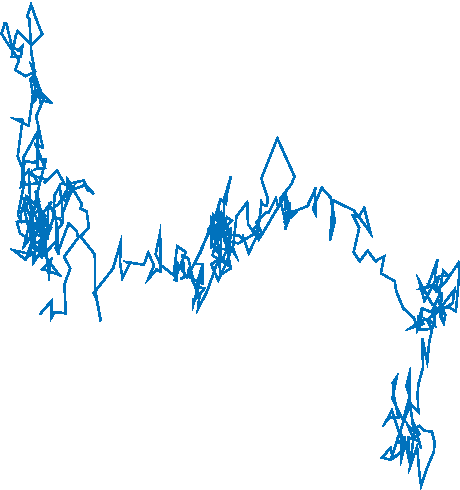
\includegraphics[height = 3cm]{./figures/mcmc/random_walk}
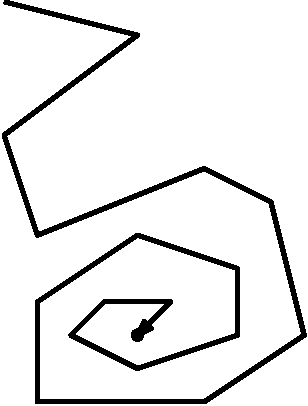
\includegraphics[height = 3cm]{./figures/mcmc/absorbing_state}
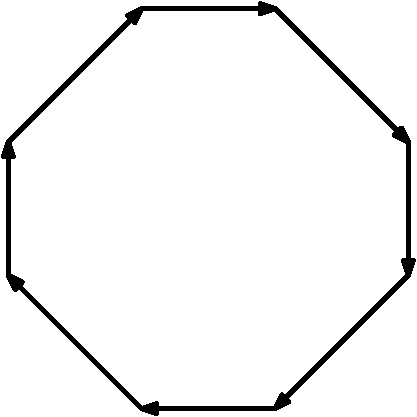
\includegraphics[height = 3cm]{./figures/mcmc/cycle}
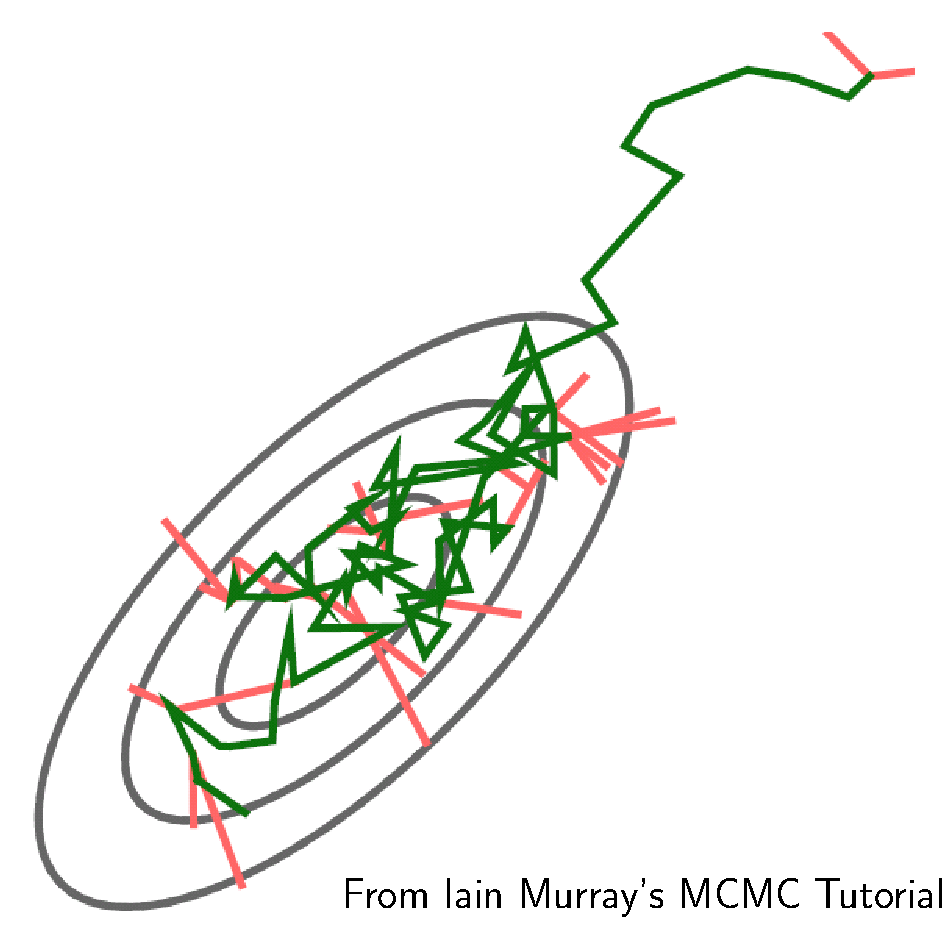
\includegraphics[height = 3cm]{./figures/mcmc/moving_to_eq_distribution}
\end{figure}

Four different behaviors of Markov chains:
\begin{itemize}[<+->]
\item Diverge (e.g., random walk diffusion where $\vec
  x\idx{t+1}\sim\gauss{\vec x\idx{t}}{\mat I}$)
\item Converge to an absorbing state
\item Converge to a (deterministic) limit cycle
\item Converge to an equilibrium distribution $p^*$: Markov chain
  remains in a region, bouncing around in a random way
\end{itemize}

\end{frame}



\begin{frame}{Example: Sampling from a uniform distribution}
\begin{figure}
\centering
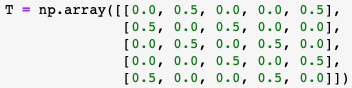
\includegraphics[height = 2.4cm]{./figures/mcmc/uniform-transition-prob}
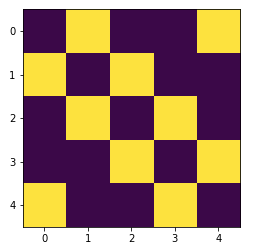
\includegraphics[height = 2.4cm]{./figures/mcmc/uniform-transition-img}
\end{figure}
Procedure:
\begin{enumerate}
\item Initialise state at $t=1$ by sampling from initial distribution $p(\vx\idx 1)$. Can be a delta function.
\item Repeat: Sample from $T(\vx\idx{t}\given \vx\idx{t-1})$
\end{enumerate}
\end{frame}



\begin{frame}{What distribution are we sampling from?}
We should ask:
\begin{center}
\Large At time $t$, what distribution are we sampling from?
\end{center}
\pause
Apply sum rule:
\begin{align*}
q(x\idx t) &= \sum_{x=1}^5 T(x\idx t | x\idx{t-1} = x) q(x\idx{t-1} = x) \\
&= \mathbf{T}\vq\idx{t-1}
\end{align*}
\pause
Why does it converge?
\begin{align*}
\vq\idx t = \mathbf{T}\vq\idx{t-1} = \mathbf{Q}\mathbf{\Lambda}\mathbf{Q}\inv \vq\idx{t-1}
\end{align*}
For this simple-to-analyse case:
\begin{itemize}
\item Only one eigenvector with $\lambda = 1$, which is $\vp$.
\item All other eigenvectors have $\lambda < 1$.
\end{itemize}
\end{frame}


%%%%%%%%%%%%%%%%%%%
% \begin{frame}

% \frametitle{Converging to an Equilibrium Distribution}

% \begin{itemize}[<+->]
% \item Remember objective: Explore/sample parameters that may have generated
% our data (generate samples from posterior)
% \\
% \arrow Bouncing around in an equilibrium distribution is a good thing
% \item Design the Markov chain such that the equilibrium distribution
%   is the desired distribution $p(\vec x)$
% \item Generate a Markov chain that converges to that equilibrium
%   distribution (independent of start state)
% \item Although successive samples are dependent we can effectively
%   generate independent samples by running the Markov chain long
%   enough: Discard most of the samples, retain only every $M$th sample
% \end{itemize}

% \end{frame}



\begin{frame}{Using Markov Chain samples: Independent chains}
If after $T$ steps, we converge to $q_{\vx\idx T}(\vx) \approx p(\vx)$.
\begin{align}
\hat{I} &\approx \frac{1}{S}\sum_{s=1}^S g(\vx_s) \,, & \vx_s \sim q(\vx\idx T) \,.
\end{align}
Where $q(\vx_T)$ is generated from the $T$th step of a Markov Chain. Time for a sample to be ``good enough'' is called \emph{burn-in time}.

\pause
\vspace{0.3cm}
\begin{itemize}
\item We run $S$ separate Markov Chains for $T$ steps. Samples are \emph{independent}, because the Markov Chains are independent.
\item Samples are approximate. May contain bias from $T$ not being large enough for the distribution to converge.
\end{itemize}
\end{frame}



\begin{frame}{Using Markov Chain samples: Single long chain}
Alternative: After $T$ steps, average all samples
\begin{align}
\hat{I} &\approx \frac{1}{S}\sum_{s=1}^S g(\vx\idx{T+s}) \,, & \vx^{(T+1)}, \dots, \vx^{(T+S)} \sim q(\vx_{T+1}, \dots, \vx_{T+S}) \,.
\end{align}
\vspace{-0.7cm}
\begin{align}
q(\vx\idx{T+1}, \dots, \vx\idx{T+S}) = q(\vx\idx T) \prod_{s=1}^{S-1} q(\vx\idx{T+s}\given \vx\idx{T+s-1})
\end{align}
\pause
\begin{itemize}
\item Remember, we choose $T$ such that $q_{\vx\idx T}(\vx) \approx p(\vx)$.
\item Only requires $T$ steps for burn-in time \emph{once}.
\item Then can get a single sample per step. However, samples are \emph{correlated}.
\end{itemize}
Usually more efficient to generate \emph{many correlated samples}, than few independent ones.
\end{frame}






\begin{frame}{Markov Chain Monte Carlo}
Markov Chain Monte Carlo estimates an integral using correlated samples from a Markov Chain. If the chain has converged, the estimate is \emph{unbiased}.
\vspace{-0.5cm}
\begin{align}
\hat{I} &\approx \frac{1}{S}\sum_{s=1}^S g(\vx^{(s)})
\end{align}
with $\{\vx^{(1)}, \vx^{(2)}, \dots\}$ from Markov Chain.
\begin{align}
\Exp{q\left(\vx^{(1)}, \vx^{(2)}, \dots\right)}{\hat I} = \frac{1}{S}\sum_{s=1}^S\Exp{q(\vx^{(s)})}{g(\vx^{(s)})} = I
\end{align} \pause
Variance decreases depending on \emph{covariance}
\begin{align*}
\Var{q(\{\vx^{(s)}\})}{\hat{I}} &= \frac{1}{S^2} \left[ \sum_{s=1}^S \Var{q(\vx\idx s)}{g(\vx\idx s)} + \sum_{t}\sum_{t'\neq t}\mathbb{C}_{q(\vx^{(t)}, \vx^{(t'))}}\left[g(\vx^{(t)}), g(\vx^{(t')})\right] \right] \nonumber \\
&= \frac{1}{S} \Var{p(\vx)}{g(\vx)} + \left[ \sum_{t}\sum_{t'\neq t}\mathbb{C}_{q(\vx^{(t)}, \vx^{(t'))}}\left[g(\vx^{(t)}), g(\vx^{(t')})\right] \right]
\end{align*}
\end{frame}


\begin{frame}{Correlation vs steps trade-off}
Independent chains:
\begin{itemize}
\item Require $T\cdot S$ transitions for $S$ samples
\item Generate independent samples, so don't need too many $S$.
\end{itemize}

\vspace{0.5cm}

Single chain:
\begin{itemize}
\item Require $T + S$ transitions for $S$ samples
\item Generates dependent samples so may need more $S$.
\end{itemize}
\end{frame}


\begin{frame}{Converging to an Equilibrium Distribution}
To get a Markov Chain that converges to a desired distribution $p(\vx)$, we need two properties:
\begin{enumerate}
\item Transition leaves $p(\vx)$ \emph{invariant}:
\begin{align}
p(\vx) = \int T(\vx|\vx') p(\vx') \calcd{\vx'}
\end{align}
i.e.~if we start with a sample from $p(\vx)$, the marginal distribution after the transition is unchanged. \pause
\item Transition is \emph{ergodic}. Definition is technical, but it is needed to ensure that $\pi(\vx^{(t)}) \to p(\vx)$ as $t\to\infty$.

Ergodic chains only have one equilibrium distribution.
\end{enumerate}
\end{frame}




% \begin{frame}
% \frametitle{Conditions for Converging to an Equilibrium Distribution}
% % If we start somewhere, chains fall into a region.  The
% % distribution where they end up will end up in an equilibrium
% % distribution, which is the distribution we are interested in.

% 2 Markov chain conditions:
% \begin{itemize}
% \item \emph{Invariance/Stationarity:} If you run the chain for a long
%   time and you are in the equilibrium distribution, you stay in
%   equilibrium if you take another step. \\
%   \arrow \cemph{Self-consistency property}
% \pause
% \item \emph{Ergodicity:} Any state can be reached from any state.\\
%   \arrow Equilibrium distribution is the same no matter where we
%   start
% %, i.e., $p(\vec
% %  x^\idx{m})\stackrel{m\to\infty}{\longrightarrow}p^*(\vec x)$.
% %\\
% %  \arrow  Be able to end up anywhere in the state space
% \end{itemize}
% \pause
% \begin{myblock}{Property}
% Ergodic Markov chains only have one equilibrium
% distribution
% \end{myblock}
% \pause

% \arrow Use ergodic and stationary Markov chains to generate samples
% from the equilibrium distribution


% % Goal: ergodicity + self-consistency.

% % Metropolis-Hastings does this.

% \end{frame}


%%%%%%%%%%%%%%%%%
\begin{frame}
\frametitle{Invariance and Detailed Balance}

% \begin{myblock}{Objective}
%   Use Markov chains to generate samples from the equilibrium
%   distribution 
% \end{myblock}

\begin{itemize}
% \item Ensure that the Markov chain is (a) ergodic, (b) leaves the
%   desired distribution invariant.
\item \cemph{Invariance:} Each step leaves the distribution $p$ invariant
  (we stay in $p$):
\begin{align*}
p(\vec x^\prime) = \sum_{\vec x} T(\vec x^\prime|\vec x)p(\vec x)
  \qquad\qquad p(\vec x^\prime) = \int T(\vec x^\prime|\vec x)
  p(\vec x) d\vec x
\end{align*}
\pause
Once we sample from $p$, the transition operator will not change
this, i.e., we do not fall back to some funny distribution $\pi\neq p$
\pause
\item \cemph{Sufficient condition} for $p$ being invariant:\\
  \emph{Detailed balance:}
\begin{align*}
p(\vec x)T(\vec x^\prime|\vec x) = p(\vec x^\prime)T(\vec x|\vec x^\prime)
\end{align*}
% \arrow Also ensures that the Markov chain is \cemph{reversible}
\end{itemize}

\end{frame}




\begin{frame}{Why is invariance not enough?}
\begin{itemize}
\item Invariance only says something about the transitions once we have \emph{reached} the stationary distribution.
\item Invariance doesn't say anything about how the chain converges.
\end{itemize}

\pause

Trivial solutions leave $p(\vx)$ invariant, e.g.~$T(\vx_{t+1}\given \vx_t) = \delta(\vx_{t+1} - \vx_t)$:
\begin{align}
\int T(\vx_{t+1} = \vx\given \vx_t = \vx') p(\vx') \calcd{\vx'} = p(\vx)
\end{align}

\pause

Ergodicity has a rather technical definition, but thankfully it is easy to guarantee!
\end{frame}






\begin{frame}{Ergodicity and communication}
A Markov Chain is ergodic if there is some probability for any state to reach any state in bounded steps. If this is true, all states are said to \emph{communicate}.

\vspace{0.3cm}


When designing Markov Chains, the easiest way to guarantee this is to have transitions that satisfy:
\begin{align}
T(\vx\idx{t+1}\given \vx\idx t) > 0 && \forall \vx\idx{t+1}, \vx\idx{t}
\end{align}

Then, all states will communicate in 1 step.
\end{frame}









\begin{frame}
\frametitle{Metropolis-Hastings}


\begin{itemize}
\item Assume that $\tilde p=Zp$ can be evaluated easily 
\item \cemph{Proposal density} $\hat T(\vec x^\prime|\vec x\idx{t})$ depends on
  last sample $\vec x\idx{t}$. \\
  Example: Gaussian with mean $\vec x\idx{t}$: $\hat T(\vec x^\prime|\vec
  x\idx{t}) = \gauss{\vec x\idx{t}}{\mat\Sigma}$
\end{itemize}
\pause
\begin{myblock}{Metropolis-Hastings Algorithm}
\begin{enumerate}
\item Generate proposal $\vec x^\prime \sim \hat T(\vec x^\prime|\vec x\idx{t})$
\item If \vspace{-5mm}
\begin{align*}
\frac{\hat T(\vec x\idx{t}|\vec x^\prime)\blue{\tilde p(\vec
  x^\prime)}}{\hat T(\vec x^\prime|\vec x\idx{t})\blue{\tilde p(\vec x\idx{t})}}
\geq u\,,\qquad u\sim U[0,1]
\end{align*}
accept the sample $\vec x\idx{t+1} = \vec x^\prime$. Otherwise set
$\vec x^{(t+1)} = \vec x\idx{t}$.
\end{enumerate}
\end{myblock}
\pause
\vspace{-1mm}
\begin{itemize}
  \item $q(\vec x\idx{t}) \stackrel{t\to\infty}{\longrightarrow}
    p(\vec x)$ \arrow Converge to equilibrium distribution
\item If proposal distribution is symmetric: \cemph{Metropolis
    Algorithm} (Metropolis et al., 1953); Otherwise
  \cemph{Metropolis-Hastings Algorithm} (Hastings, 1970)\nocite{Metropolis1953,Hastings1970}
\end{itemize}

\end{frame}
%%%%%%%%%%%%%%%%%%%%%%%%%%%%%%%%%%%%%%%%%%%%%%%%%%%%%%
\begin{frame}
\frametitle{Example}
\begin{figure}
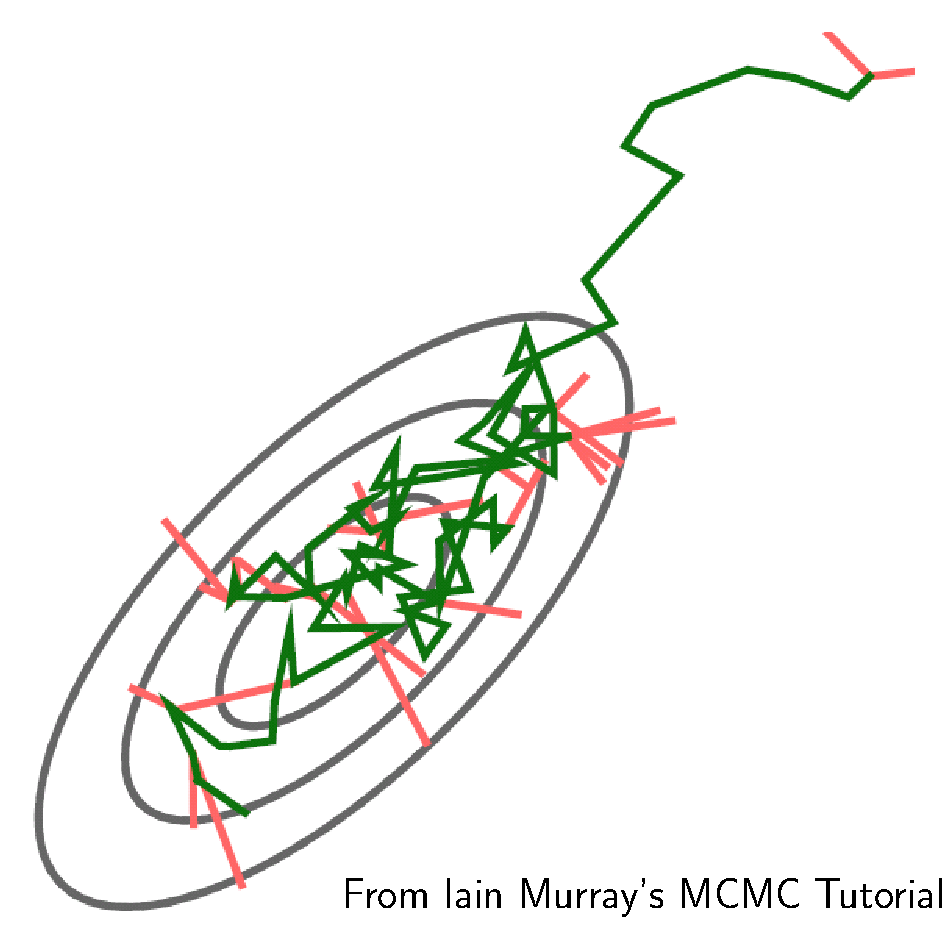
\includegraphics[height = 7cm]{./figures/mcmc/moving_to_eq_distribution}
\end{figure}
\end{frame}

%%%%%%%%%%%%%%%%%%%%%%%%%%%%%%%%%%%%%%%%%%%%%%%%%%%%%%
\begin{frame}
\frametitle{Step-Size Demo}


\begin{itemize}
\item Explore $p(x)=\gaussx{x}{0}{1}$ for different step sizes $\sigma$. 
\item We can only evaluate $\log \tilde p(x) = -x^2/2$
\item Proposal distribution $q$: Gaussian
  $\gaussx{x\idx{t+1}}{x\idx{t}}{\sigma^2}$ centered at the current
  state for various step sizes $\sigma$
\item Expect to explore the space between $-2,2$ with high probability 
\end{itemize}

\end{frame}
%%%%%%%%%%%%%%%%%%%%%%%%%%%%%%%%%%%%%%%%%%%%%%%%%%%%%% 

\begin{frame}
\frametitle{Step-Size Demo: Discussion}
\begin{itemize}[<+->]
\item Acceptance rate depends on the step size of the proposal distribution \\
  \arrow Exploration parameter
\item If we do not reject enough, the method does not work. 
\item In rejection sampling we do not like rejections, but in MH
  rejections tell you where the target distribution is.
\item Theoretical results: in 1D 44\%, in higher dimensions about 25\%
  acceptance rate for good mixing properties
\item Tune the step size
\end{itemize}
\end{frame}

%%%%%%%%%%%%%%%%%%%%%%%%%%%%%%%%%%%%%%%%%%%%%%%%%%%%%%

\begin{frame}
\frametitle{Properties}
\begin{itemize}
\item Samples are correlated \\
\pause
\item If $\hat T>0$ everywhere, we will end up in the \cemph{equilibrium
    distribution:}
  $\pi(\vec x\idx{t}) \stackrel{t\to\infty}{\longrightarrow} p^*(\vec
  x)$ \pause
\item Explore the state space by random walk\\
\arrow May take many steps, if the steps are short compared to the distribution
\item No further catastrophic problems in high dimensions
%\item Convergence difficult to assess
\end{itemize}

\end{frame}






% \begin{frame}
% \frametitle{Gibbs Sampling (Geman \& Geman, 1984)\nocite{Geman1984}}
% \begin{itemize} 
% \item Assumption: $p(\vec x) = p(x_1,\dotsc,x_n)$ is too complicated
%   to draw samples from directly, but \cemph{its conditionals
%     $p(x_i|\vec x_{\backslash i})$ are tractable to work with}
% \item Any distribution ``with a name'' (Gaussian, Laplace, Bernoulli,
%   Gamma, Wishart, ...) is easy to sample from
%   (standard libraries)
% \pause
% \item Trick: Update that always accepts
% \item No need to tune step-length
% \end{itemize}
% \end{frame}

% %%%%%%%%%%%%%%%%%%%%%%%%%%%%%%%%%%%%%%%%%%%%%%%%%%%%%%

% \begin{frame}
%   \frametitle{Algorithm} 

% \begin{columns}
% \column{0.55\hsize}

% Assuming $n$ parameters $x_1,\dotsc, x_n$,
%   Gibbs sampling samples individual variables conditioned on all
%   others:

% \begin{enumerate}
% \item $x_1^\idx{t+1}\sim p(x_1|x_2^\idx{t},\dotsc, x_n^\idx{t})$
% \item $x_2^\idx{t+1}\sim p(x_2|x_1^\idx{t+1}, x_3^\idx{t}, \dotsc,
%   x_n^\idx{t})$
% \item $\vdots$
% \item $x_n^\idx{t+1}\sim p(x_n|x_1^\idx{t+1},\dotsc, x_{n-1}^\idx{t+1})$
% \end{enumerate}
% \column{0.4\hsize}
% \begin{figure}
% \centering
% 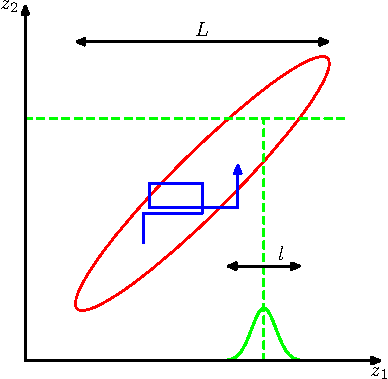
\includegraphics[width = \hsize]{./figures/mcmc/Figure11_11}\\
% \tiny{From PRML (Bishop, 2006)}
% \end{figure}
% \end{columns}
% \end{frame}








% % \begin{frame}
% % \frametitle{}
% % %% Composition of transition operators T_A is a valid transition operator
% % %% Gibbs sampling is an example of this: T_A only explores 1 variable, T_B the other one. For discrete it's easy; for continuous more tricky. If the conditional distribution "has a name", we can use a library. Does requires some maths. WinBUGS, STAN, JAGS derives the conditionals of the model for you, and it works out how to do the updates. No choice of stepsize required. Fallback: Metropolis 
% % \begin{itemize}
% % \item Gibbs sampling may not work well if the variables are correlated.
% % \newline
% % \arrow Transform the space (e.g., Adaptive Direction Sampling)\newline
% % \arrow Blocking/Collapsing (update more than 1 variable at once) % 1:18 in video
% % \item Probabilistic programming makes various choices for you. 
% % \item Auxiliary variable MCMC (e.g., Slice, Swendsen-Wang, HMC, ...)
% % \end{itemize}
% % \end{frame}
% %%%%%%%%%%%%%%%%%%%%%%%%%%%%%%%%%%%%%%%%%%%%%%%%%%%%%%
% \begin{frame}
% \frametitle{Gibbs Sampling: Ergodicity}
% \begin{figure}
% \centering
% 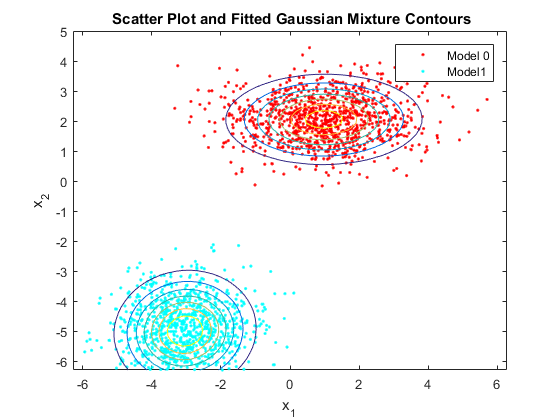
\includegraphics[height = 3.5cm]{./figures/mcmc/gibbs_hard_time}
% \end{figure}

% \begin{itemize}
% \item $p(\vec x)$ is invariant
% \item \cemph{Ergodicity:} Sufficient to show that all conditionals are
%   greater than 0. \\
%   \arrow Then any point in $x$-space can be reached from any other
%   point (potentially with low probability) in a finite number of steps
%   involving one update of each of the component variables.
% \end{itemize}
% \end{frame}

% %%%%%%%%%%%%%%%%%%%%%%%%%%%%%%%%%%%%%%%%%%%%%%%%%%%%%%
% \begin{frame}
% \frametitle{Finding the Conditionals}
% \begin{enumerate}
% \item Write down the (log-) joint distribution $p(x_1,\dotsc, x_n)$
% \item For each $x_i$
% \begin{enumerate}
% \item Throw away all terms that do not depend on the current sampling variable
% \item Pretend this is the density for your variable of interest and all other variables are fixed. What distribution does the log-density remind you of?
% \item That is your conditional sampling density $p(x_i|\vec
%   x_{\backslash i})$
% \end{enumerate}
% \end{enumerate}
% \end{frame}

% %%%%%%%%%%%%%%%%%%%%%%%%%%%%%%%%%%%%%%%%%%%%%%%%%%%%%% 

% \begin{frame}
% \frametitle{Example}
% \begin{itemize}
% \item Model:
% \begin{align*}
% &y_i \sim \gauss{\mu}{\tau\inv}\,,\quad 
% \mu \sim \gaussx{\mu}{0}{1}\,,\quad
%       \tau \sim \text{Gamma}(\tau | 2,1)\\
%   &\text{Gamma}(\tau|2,1) =   \frac{1}{\Gamma(2)}\tau \exp(-\tau)
% \end{align*}
% %\vspace{-10mm}
% \item \textbf{Objective:} Generate samples from the parameter
%   posterior $p(\mu, \tau|y_1,\dotsc, y_N)$ given $N$ observations
%   $y_1, \dotsc, y_N$
% \pause
% \item Then
% \begin{align*}
% p(\vec y,\mu,\tau) &= \prod\nolimits_{i=1}^N p(y_i|\mu, \tau)p(\mu)p(\tau)\\
% &\propto
%   \tau^{N/2}\exp(-\frac{\tau}{2}\sum\nolimits_i(y_i-\mu)^2)\exp(-\tfrac{1}{2}\mu^2)\tau\exp(-\tau)\\
% \onslide+<3->{
% p(\mu|\tau, \vec y) &= \gaussx{\mu}{\tfrac{\tau\sum\nolimits_i y_i}{1+N\tau}}{(1+N\tau)\inv}\\
% p(\tau|\mu, \vec y) &= \text{Gamma}(\tau | 2+\tfrac{N}{2},
%               1+\tfrac{1}{2}\sum\nolimits_i (y_i - \mu)^2)
% }
% \end{align*}
% \end{itemize}
% \end{frame}



% %%%%%%%%%%%%%%%%%%%%%%%%%%%%%%%%%%%%%%%%%%%%%%%%%%%%%%

% \begin{frame}
% \frametitle{Gibbs Sampling: Properties}
% \begin{itemize}[<+->]
% \item Gibbs is Metropolis-Hastings with acceptance
%   probability 1:\\
%   Sequence of proposal distributions $q$ is defined in terms of
%   \underline{conditional} distributions of the joint $p(\vec x)$
%   \\
%   \arrow \cemph{Converge} to equilibrium distribution: $p^\idx{t}(\vec
%   x)\stackrel{t\to\infty}{\longrightarrow} p(\vec x)$\\
%   \arrow Exploration by random walk behavior can be slow
% \item \cemph{No adjustable parameters} (e.g., step size)%: Automatically governed by the conditional distribution
% \item Applicability depends on how easy it is to draw samples from the
%   conditionals
% \item May not work well if the \calert{variables are correlated}
% % \\
% % \arrow Blocking/Collapsing (update more than 1 variable at once) \\% 1:18 in video
% % \arrow Auxiliary variable MCMC (e.g., Slice, Swendsen-Wang, HMC, ...)
% \item \cemph{Statistical software} derives the conditionals of the
%   model, and it works out how to do the updates:
%   STAN\footnote{\url{http://mc-stan.org/}},
%   WinBUGS\footnote{\url{http://www.mrc-bsu.cam.ac.uk/software/bugs/}},
%   JAGS\footnote{\url{http://mcmc-jags.sourceforge.net/}}
% \end{itemize}

% \end{frame}

%%%%%%%%%%%%%%%%%%%%%%%%%%%%%%%%%%%%%%%%%%%%%%%%%%%%%%
% \begin{frame}
% \frametitle{Flavors of Gibbs Sampling}
% \begin{itemize}
% \item \cemph{Collapsed Gibbs sampler:} Analytically integrate out some
%   parameters and sample the rest.\newline
% \arrow Tends to be much more efficient with smaller variance \\(see
% Rao-Blackwellization in the state estimation literature)\nocite{Liu1994}
% \item \cemph{Block-Gibbs sampler:} Sample groups of variables at a
%   time instead of single-site updating
% \end{itemize}

% \end{frame}



% \input{mcmc_analysis}


\begin{frame}
\frametitle{MCMC Diagnostics: Trace Plots}
\begin{figure}
\centering
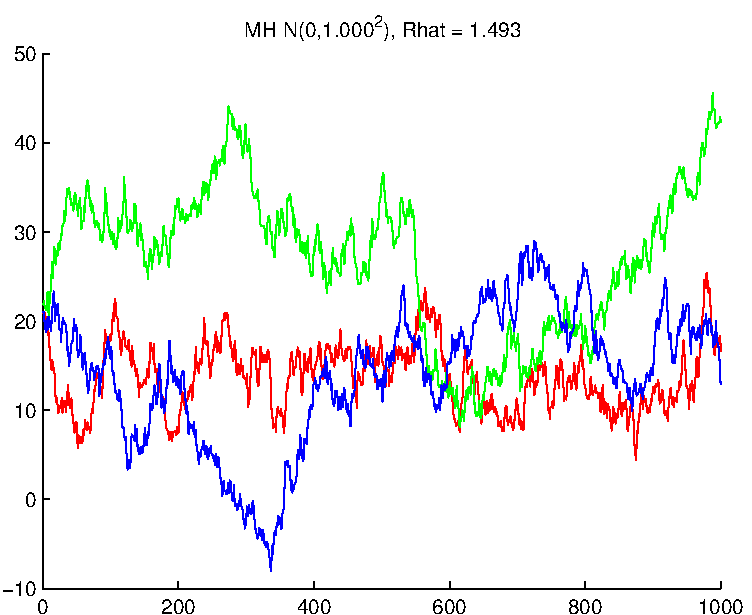
\includegraphics[height = 3cm]{./figures/mcmc/mcmcGmmDemoSigma1-traceplot}
\hspace{5mm}
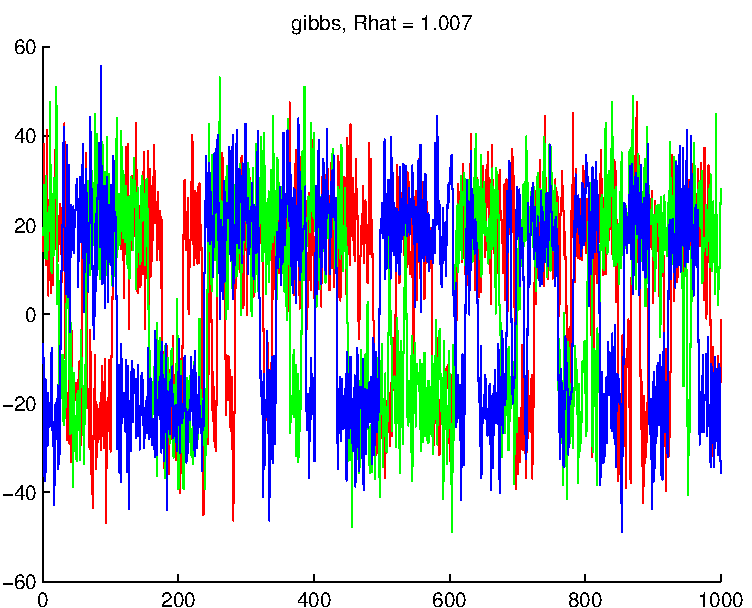
\includegraphics[height = 3cm]{./figures/mcmc/mcmcGmmDemoSigma0-traceplot}
\\[2mm]
{\small Figure from Murphy (2012)\nocite{Murphy2012}}
\end{figure}
\begin{itemize}
\item  \cemph{Mixing time:} Amount of time it takes the Markov chain to
  converge to the stationary distribution and forget its initial
  state.
\item \cemph{Trace plots:} Run multiple chains from very different starting
  points, plot the samples of the variables of interest. If the chain
  has mixed, the trace plots should converge to the same distribution.
\end{itemize}

\end{frame}


\begin{frame}
  \frametitle{Summary}

  \begin{itemize}
  \item MCMC generates a Markov chain of dependent samples that allow
    us to generate samples from the target distribution
  \item Metropolis Hastings algorithm
  \end{itemize}
\end{frame}



\begin{frame}{Further Reading}
\begin{itemize}
\item MacKay, ch 29
\item Murphy, ch 24
\end{itemize}
\end{frame}









%%%%%%%%%%%%%%%%%%%%%%%%%%%%%%%%%%%%%%%%%
% REFERENCES
%%%%%%%%%%%%%%%%%%%%%%%%%%%%%%%%%%%%%%%%%
\begin{frame}[t,allowframebreaks]
\frametitle{References}
\linespread{1.0}
\tiny
\bibliographystyle{abbrv}
\bibliography{../includes/pi-literature}
\end{frame}



\end{document}
%%% Local Variables: 
%%% mode: latex
%%% TeX-master: t
%%% End: 
